\section{Match Statement} %%%%%%%%%%%%%%%%%%%%%%%%%%%%%%%%%%%%%%%%%%%%%%%%%%%%%%%
\label{sec:impl}

Our implementation of pattern matching expressions follows the naive way of 
essentially interpreting them through backtracking. On one hand, this was a 
consequence of working in a library setting, where code transformations are much 
harder to achive. On the other hand, from the very beginning we were trying to 
find an expressive alternative to object decomposition with either nested 
dynamic casts or visitor design pattern, and thus were not concerned with 
pattern matching on multiple arguments, where decision tree approach becomes 
more efficient. Dealing with single argument certainly leaves less choices for 
optimization, but does not eliminate them as repeated use of constructor-pattern 
with the same target type but different argument patterns essentially leads to 
the same inefficiencies. To tackle this issue in a library setting we rely on 
and give more control to the library user. For example, we fix the order of 
evaluation, but let guard-patterns be placed directly on the arguments of a 
constructor-pattern to let the user benefit from the consciesness of expression, 
while holding a grip on performance. Similarly, we added \code{Alt} sub-clauses 
to \code{Qua}-clause to syntactically separate fast type switching from slow 
sequential evaluation of pattern matching expressions. The fall-through behavior 
of the \code{Match}-statement allows the user to achieve the same effect 
directly with \code{Qua}-clauses, however the performance overhead involved 
justified the addition of otherwise syntactic sugar.

The interpretation of pattern matching expressions with expression templates follows 
very closely the composition of expressions described by abstract syntax 
in~\textsection\ref{sec:syn} as well as their application to subject expression 
described by evaluation rules in \textsection\ref{sec:semme}. This section thus
mainly concentrates on efficient implementation of a match statement as 
well as unification of its syntax to the three encodings of algebraic data types
outlined in \textsection\ref{sec:adt}. The discussion will largely focus on 
devising an efficient \emph{type-switch}, which is then used by our library as a 
backbone to the general match statement presented in~\textsection\ref{sec:semms}. 

By encoding algebraic data types with classes we alter their semantics in two 
important ways: we make them \emph{extensible} as new variants can be added by 
simply deriving from the base class, as well as \emph{hierarchical} as variants 
can be inherited from other variants and thus form a subtyping relation between 
themselves~\cite{Glew99}. This is not the case with traditional algebraic data 
types in functional languages, where the set of variants is \emph{closed}, while 
the variants are \emph{disjoint}. Some functional languages e.g. 
ML2000~\cite{ML2000} and Moby~\cite{Moby} were experimenting with 
\emph{hierarchical extensible sum types}, which are closer to object-oriented 
classes then algebraic data types are, but, interestingly, they did not provide 
pattern matching facilities on them. Working within a multi-paradigm  
programming language like C++, we will not be looking at algebraic data types in
the closed form they are present in functional languages, but rather in an 
open/extensible form discussed by Zenger~\cite{Zenger:2001}, Emir~\cite{EmirThesis}, 
L\"oh~\cite{LohHinze2006}, Glew~\cite{Glew99} and others. We will thus 
assume an object-oriented setting where new variants can be added later and form
subtyping relations between each other including those through multiple 
inheritance. We will look separately at polymorphic and tagged class encodings 
as our handling of these two encodings is significantly different. Before we 
look into these differences in greater details, however, we would like to look 
at the problem of type switching without specific implementation in mind as well 
as properties we would like to seek from such an implementation.

\subsection{Type Switch}

Functional languages use pattern matching to perform case analysis on a given 
algebraic data type. In this section we will try to generalize this construct to 
case analysis of hierarchical and extensible data types. Presence of such a
construct will allow for external function definitions by detaching a particular 
case analysis from the hierarchy it is performed on.

Consider a class \code{B} and a set of classes \code{Di} directly or indirectly 
inherited from it. An object is said to be of the \emph{most derived type} 
\code{D} if it was created by explicitly calling a constructor of that type.
The inheritance relation on classes induces a subtyping relation on them, which in 
turn allows objects of a derived class to be used in places where an object of a 
base class is expected. The type of variable or parameter referencing such an
object is called the \emph{static type} of the object. When object is passed by 
reference or by pointer, we might end up in a situation where the static type of an 
object is different from its most derived type, with the latter necessarily 
being a subtype of the former. The most derived class along with all its base classes 
that are not base classes of the static type are typically referred to as the 
\emph{dynamic types} of an object. At each program point the compiler knows the 
static type of an object, but not its dynamic types.

By \emph{type switch} we will call a control structure taking either a pointer 
or a reference to an object, called \emph{subject}, and capable of uncovering a 
reference or a pointer to a full object of a type present in the list of case 
clauses. Similar control structures exist in many programming languages and 
date back to at least Simula's Inspect statement~\cite{Simula67}.

Consider an object of (most derived) type \code{D}, pointed to by a variable of 
static type \code{B*}: e.g. \code{B* base = new D;}. A hypothetical type switch 
statement, not currently supported by C++, can look as following:

\begin{lstlisting}
switch (base)
{
    case D1: s1;
    ...
    case Dn: sn;
}
\end{lstlisting}

\noindent and can be given numerous plausible semantics:

\begin{itemize}
\setlength{\itemsep}{0pt}
\setlength{\parskip}{0pt}
\item \emph{First-fit} semantics will evaluate the first statement $s_i$ such 
      that $D_i$ is a base class of $D$
\item \emph{Best-fit} semantics will evaluate the statement corresponding to the 
      most derived base class $D_i$ of $D$ if it is unique (subject to 
      ambiguity)
\item \emph{The-only-fit} semantics will only evaluate statement $s_i$ if $D_i=D$.
\item \emph{All-fit} semantics will evaluate all statements $s_i$ whose guard 
      type $D_i$ is a subtype of $D$ (order of execution has to be defined)
\item \emph{Any-fit} semantics might choose non-deterministically one of the 
      statements enabled by all-fit
\end{itemize}

\noindent
The list is not exhaustive and depending on a language, any of these semantics 
or their combination might be a plausible choice. Functional languages, for 
example, often prefer first-fit, while object-oriented languages would typically 
be inclined to best-fit semantics. The-only-fit semantics is traditionally seen 
in procedural languages like C and Pascal to deal with discriminated union types. 
All-fit and any-fit semantics might be seen in languages based on predicate 
dispatching~\cite{ErnstKC98} or guarded commands~\cite{EWD:EWD472}, where a 
predicate can be seen as a characteristic function of a type, while logical 
implication can be seen as subtyping.

\subsection{Open and Efficient Type Switching}
\label{sec:poets}

The fact that algebraic data types in functional languages are closed allows for 
their efficient implementation. The traditional compilation scheme assigns unique 
tags to every variant of the algebraic data type and pattern matching is then 
simply implemented with a jump table over all tags. A number of issues in 
object-oriented languages makes this extremely efficient approach infeasible:

\begin{itemize}
\setlength{\itemsep}{0pt}
\setlength{\parskip}{0pt}
\item Extensibility
\item Subtyping
\item Multiple inheritance
\item Separate compilation
\item Dynamic linking 
\end{itemize}

\noindent
Unlike functional style algebraic data types, classes are \emph{extensible} 
whereby new variants can be arbitrarily added to the base class in the form of 
derived classes. Such extension can happen in a different translation unit or a
static library (subject to \emph{separate compilation}) or a dynamically linked 
module (subject to \emph{dynamic linking}). Separate compilation effectively 
implies that all the derived classes of a given class will only be known at link 
time, postponing thus any tag-allocation related decisions until then. The 
Presence of dynamic linking effectively requires the compiler to assume that the 
exact derived classes will only be known at run time, and not even at start-up 
time.

%and thus any tag allocation scheme should on one hand assume presence of 
%unknown tags and on the other -- the necessity of maintaing the same tags for 
%the commonly seen classes of each dynamic module.  

The \emph{subtyping} relation that comes along with extensibility through 
subclassing effectively gives every class multiple types -- its own and the 
types of all its base classes. In such a scenario it is natural to require that 
type switching can be done not only against the exact dynamic type of an object, 
but also against any of its base classes (subject to our substitutability 
requirement). This in itself is not a problem for functional-style tag 
allocation as long as the set of all derived classes is known, since the 
compiler can partition tags of all the derived classes according to chosen 
semantics based on classes mentioned in case clauses.
Unfortunately this will not work in the presence of dynamic linking as there 
might be new derived classes with tags not known at the time of partitioning and 
thus not mentioned in the generated jump table.

\emph{Multiple inheritance} complicates things further by making each class 
potentially belong to numerous unrelated hierarchies. Any tag allocation scheme 
capable of dealing with multiple inheritance will either have to assure that 
generated tags satisfy properties of each subhierarchy independently or use 
different tags for different subhierarchies. Multiple inheritance also 
introduces such a phenomenon as \emph{cross-casting}, whereby a user may request 
to cast pointers between unrelated classes, since they can potentially become 
base classes of a later defined class. From an implementation point of view this 
means that not only do we have to be able to check that a given object belongs 
to a given class (type testing), but also be able to find a correct offset to it 
from a given base class (type casting).

While looking at various schemes for implementing type switching we noted down a 
few questions that might help evaluate and compare solutions: 

\begin{enumerate}
\setlength{\itemsep}{0pt}
\setlength{\parskip}{0pt}
\item Can the solution handle base classes in case clauses?
\item Will it handle the presence of base and derived classes in the same match statement?
\item Will it work with derived classes coming from a DLL?
\item Can it cope with multiple inheritance (repeated, virtual)?
\item Can independently developed DLLs that either extend classes involved in 
      type switching or do type switching themselves be loaded together without 
      any integration efforts?
\item Are there any limitations on the number and or shape of class extensions?
\item What is the complexity of performing matching, based on the number of case clauses and 
      the number of possible types?
\end{enumerate}

The number of possible types in the last question refers to the number of subtypes 
of the static type of the subject, not all the types in the program. Several 
solutions discussed below depend on the number of case clauses in the match 
statement, which raises the question of how many such clauses a typical program 
might have. The C++ pretty-printer for Pivot we implemented using our pattern 
matching techniques originally had 8 match statements with 5, 7, 8, 10, 15, 17, 30 
and 63 case clauses each. While experimenting 
with probability distributions of various classes to minimize the number of 
conflicts (see \textsection\ref{sec:moc}), we had to associate probabilities 
with classes and implemented it with a match statement over all 160 nodes in the 
Pivot's class hierarchy. With Pivot having the smallest number of node kinds 
among the compiler frameworks we had a chance to work with, we expect a similar 
or larger number of case clauses in other compiler applications.

Instead of starting with an efficient solution and trying to make it open, let us 
start with an open solution and try to make it efficient. 
An obvious solution that will pass the above checklist can look like the following:

\begin{lstlisting}
if (D1* derived = dynamic_cast<D1*>(base)) { s1; } else
if (D2* derived = dynamic_cast<D2*>(base)) { s2; } else
...
if (Dn* derived = dynamic_cast<Dn*>(base)) { sn; }
\end{lstlisting}

\noindent
Despite the obvious simplicity, its main drawback is performance: a typical 
implementation of \code{dynamic_cast} might take time proportional to the 
distance between base and derived classes in the inheritance tree~\cite{XXXXX}.
What is worse, is that the time to uncover the type in the $i^{th}$ case clause 
is proportional to $i$, while failure to match will always take the longest. 
This linear increase can be seen in the Figure~\ref{fig:DCastVis1}, where 
the above cascading-if was applied to a flat hierarchy encoding an algebraic 
data type with 100 variants. The same type-switching functionality implemented 
with the visitor design pattern took only 28 cycles regardless of the 
case.\footnote{Each case $i$ was timed multiple times, thus turning the experiment 
into a repetitive benchmark described in \textsection\ref{sec:eval}. In a more
realistic setting, represented by random and sequential benchmarks, the cost of 
double dispatch was varying between 52 and 55 cycles.}
This is more than 3 times faster than the 93 cycles it took to uncover even the 
first case with \code{dynamic_cast}, while it took 22760 cycles to uncover the 
last.

\begin{figure}[htbp]
  \centering
    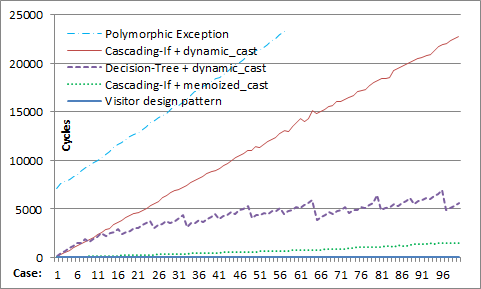
\includegraphics[width=0.47\textwidth]{DCast-vs-Visitors1.png}
  \caption{Type switching based on na\"ive techniques}
  \label{fig:DCastVis1}
\end{figure}

When the class hierarchy is not flat and has several levels, the above cascading-if can be replaced 
with a decision tree that tests base classes first and thus eliminates many of 
the derived classes from consideration. This approach is used by Emir to deal with 
type patterns in Scala~\cite[\textsection 4.2]{EmirThesis}. The intent is to 
replace a sequence of independent dynamic casts between classes that are far 
from each other in the hierarchy with nested dynamic casts between classes that 
are close to each other. Another advantage is the possibility to fail early: 
if the type of the subject does not match any of the clauses, we will not have to try all the cases. 
A flat hierarchy, which will likely be formed by the leaves in even a multi-level 
hierarchy, will not be able to benefit from this optimization and 
will effectively degrade to the above cascading-if. Nevertheless, when 
applicable, the optimization can be very useful and its benefits can be seen in
Figure~\ref{fig:DCastVis1} under ``Decision-Tree + dynamic\_cast''. The class 
hierarchy for this timing experiment formed a perfect binary tree with 
classes number 2*N and 2*N+1 derived from a class with number N. The structure 
of the hierarchy also explains the repetitive pattern of timings.

The above solution either in a form of cascading-if or as a decision tree can be 
significantly improved by lowering the cost of a single \code{dynamic_cast}. 
We devised an asymptotically constant version of this operator that we call
\code{memoized_cast} in \textsection\ref{sec:memcast}. As can be seen 
from the graph titled ``Cascading-If + memoized\_cast'', it speeds up the 
above cascading-if solution by a factor of 18 on average, as well as outperforms 
the decision-tree based solution with dynamic\_cast for a number of case clauses 
way beyond those that can happen in a reasonable program. 
We leave the discussion of the technique until 
\textsection\ref{sec:memcast}, while we keep it in the chart to give perspective on 
an even faster solution to dynamic casting. The slowest implementation in the 
chart based on exception handling facilities of C++ is discussed in 
\textsection\ref{sec:xpm}.

The approach of Gibbs and Stroustrup~\cite{FastDynCast} employs divisibility of numbers to obtain a 
tag allocation scheme capable of performing type testing in constant time. 
Extended with a mechanism for storing offsets required for this-pointer 
adjustments, the technique can be used for extremely fast dynamic casting on 
quite large class hierarchies. The idea is to allocate tags 
for each class in such a way that tag of a class D is divisible by a tag of a 
class B if and only if class D is derived from class B. For comparison purposes 
we hand crafted this technique on the above flat and binary-tree hierarchies and 
then redid the timing experiments from Figure~\ref{fig:DCastVis1} using the fast 
dynamic cast. The results are presented in Figure~\ref{fig:DCastVis2}. For 
reference purposes we retained ``Visitor Design Pattern'' and ``Cascading-If + 
memoized\_cast'' timings from Figure~\ref{fig:DCastVis1} unchanged. Note that 
the Y-axis has been scaled-up 140 times, which is why the slope of 
``Cascading-If + memoized\_cast'' timings is so much steeper.

\begin{figure}[htbp]
  \centering
    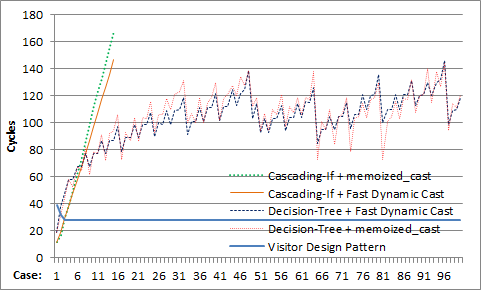
\includegraphics[width=0.47\textwidth]{DCast-vs-Visitors2.png}
  \caption{Type switching based on the fast dynamic cast of Gibbs and Stroustrup~\cite{FastDynCast}}
  \label{fig:DCastVis2}
\end{figure}

As can be seen from the figure the use of our memoized\_cast implementation can 
get close in terms of performance to the fast dynamic cast, especially 
when combined with decision trees. An important difference that cannot be seen 
from the chart, however, is that the performance of memoized\_cast is 
asymptotic, while the performance of fast dynamic cast is guaranteed. This 
happens because the implementation of memoized\_cast will incur an overhead of 
a regular dynamic\_cast call on every first call with a given most derived type. 
Once that class is memoized, the performance will remain as shown. Averaged over 
all calls with a given type we can only claim we are asymptotically as good as 
fast dynamic cast.

Unfortunately fast dynamic casting is not truly open to fully satisfy our 
checklist. The structure of tags required by the scheme limits the number of 
classes it can handle. A 32-bit integer is estimated to be able to represent 7 
levels of a class hierarchy that forms a binary tree (255 classes), 6 levels of 
a similar ternary tree hierarchy (1093 classes) or just one level of a hierarchy 
with 9 base classes -- multiple inheritance is the worst case scenario of the 
scheme that quickly drains its allocation possibilities. Besides, similarly to 
other tag allocation schemes, presence of class extensions in \emph{Dynamically Linked Libraries} (DLLs) will likely 
require an integration effort to make sure different DLLs are not reusing prime 
numbers in a way that might result in an incorrect dynamic cast.

A number of other constant-time techniques for class-membership testing is 
surveyed by Gil and Zibin~\cite[\textsection 4]{PQEncoding}. They are intended 
for type testing, and thus will have to be combined with decision trees 
for type switching, resulting in similar to fast dynamic cast performance. 
They too assume access to the entire class hierarchy at compile time and thus 
are not open.

In view of the predictably-constant dispatching overhead of the visitor design pattern, 
it is clear that any open solution that will have a non-constant dispatching 
overhead will have a poor chance of being adopted. Multi-way switch on 
sequentially allocated tags~\cite{Spuler94} was one of the few techniques that 
could achieve constant overhead, and thus compete with and even outperform visitors. 
Unfortunately the scheme has problems of its own that make it unsuitable for 
truly open type-switching and here is why.

%To better understand the problem let us look at some existing solutions to type 
%switching that we found to be used in practice. 

%From our experience on this project we have noticed that we can only compete 
%with visitors when switch statements are implemented with a jump table. As soon 
%as compiler was putting even a single branch into the decision tree of cases, 
%the performance was degraded significantly. From this perspective we do not 
%regard solutions based on decision trees as efficient, since they do not let us 
%compete compete with the visitors solution.

The simple scheme of assigning a unique tag per variant (instantiatable class 
here) will not pass our first question because the tags of base and derived 
classes will have to be different if the base class can be instantiated on its 
own. In other words we will not be able to land on a case label of a base class, while 
having a derived tag only. The already mentioned partitioning of tags of derived 
classes based on the classes in case clauses also will not help as it assumes 
knowledge of all the classes and thus fails extensibility through DLLs.

In practical implementations hand crafted for a specific class hierarchy, tags 
often are not chosen arbitrarily, but to reflect the subtyping relation of the 
underlying hierarchy. Switching on base classes in such a setting will typically 
involve a call to some function $f$ that converts derived class' tag into a base 
class' tag. An example of such a scheme would be having a certain bit in the tag 
set for all the classes derived from a given base class. Unfortunately this 
solution creates more problems than it solves.

First of all the solution will not be able to recognize an exceptional case 
where most of the derived classes should be handled as a base class, while a few 
should be handled specifically. Applying the function $f$ puts several different 
types into an equivalence class with their base type, making them 
indistinguishable from each other.

Secondly, the assumed structure of tags is likely to make the set of tags 
sparse, effectively forcing the compiler to use a decision tree instead of a jump 
table to implement the switch. Even though conditional jump is reported to be 
faster than indirect jump on many computer architectures~\cite[\textsection 
4]{garrigue-98}, this did not seem to be the case in our experiments. Splitting 
of a jump table into two with a condition, that was sometimes happening because 
of our case label allocation scheme, was resulting in a noticeable degradation of 
performance in comparison to a single jump table.

Besides, as was seen in the scheme of Gibbs and Stroustrup, the assumed 
structure of tags can also significantly decrease the number of classes a given 
allocation scheme can handle. It is also interesting to note that even though 
their scheme can be easily adopted for type switching with decision trees, it is 
not easily adoptable for type switching with jump tables: in order to obtain 
tags of base classes we will have to decompose the derived tag into primes and 
then find all the dividers of the tag present in case clauses.

To summarize, truly open and efficient type switching is a non-trivial problem. 
The approaches we found in the literature were either open or efficient, 
but not both. Efficient implementation was typically achieved by sealing the 
class hierarchy and using a jump table on sequential tags. Open implementations 
were resorting to type testing and decision trees, which was not efficient. 
We are unaware of any efficient tag allocation scheme that can be used in a 
truly open scenario.

%%%%%%%%%%%%%%%%%%%%%%%%%%%%%%%%%%%%%%5555

%\noindent
%We chose to give it a first-fit semantics in our library as it was resembling 
%pattern matching facilities of other languages and was the most intuitive. The 
%following code can be generated to implement it:
%
%\begin{lstlisting}
%if (D1* derived = dynamic_cast<D1*>(base)) { s1; } else
%if (D2* derived = dynamic_cast<D2*>(base)) { s2; } else
%...
%if (Dn* derived = dynamic_cast<Dn*>(base)) { sn; }
%\end{lstlisting}

%\noindent
%Note that leaving \code{else} out will effectively turn it into an all-fit 
%statement with enabled statements executed in lexicographical order.
%
%The above code is easy to understand but is extremely inefficient as for an 
%object of dynamic type $D_i$ we will have to perform $i-1$ dynamic casts that 
%fail first. The diagram below compares the times spent by visitors and the above 
%type switch statement to uncover the $i^{th}$ case. We postpone the discussion 
%of \code{memoized_cast} until section \textsection\ref{}, here we would only 
%like to notice that even though faster than the actual dynamic cast it also bears 
%a linear coefficient, not present in visitors.

\section{Solution for Polymorphic Classes}
\label{sec:copc}

Our handling of type switches for polymorphic and tagged encodings differs 
with each having its pros and cons described in details in \textsection\ref{sec:cmp}.
In this section we will concentrate on the truly open type switch for 
polymorphic encoding. The type switch for tagged encoding (\textsection\ref{sec:cotc}) 
is simpler and more efficient, however, making it open will eradicate its 
performance advantages. The difference in performance is the price we pay for 
keeping the solution open.  The core of the proposal relies on two key
aspects of C++ implementations:
\begin{enumerate}
\item a constant-time access to the virtual table pointer embedded in an object of
  dynamic class type;
\item injectivity of the relation between an object's inheritance path
  and the virtual table pointer extracted from that object.
\end{enumerate}

\subsection{Virtual Table Pointers}
\label{sec:vtp}

Before we discuss our solution we would like to talk about certain properties of 
the C++ run-time system that we rely on. In particular,
we show that under certain conditions the compiler cannot share 
the same virtual tables between different classes or subobjects of the same 
class. This allows us to use virtual table pointers to \emph{uniquely} identify 
the subobjects within the most derived class.

Strictly speaking, the C++ standard~\cite{C++0x} does not require implementations 
to use any specific technique (e.g. virtual tables) to implement virtual functions, 
however interoperability requirements have forced many compiler vendors to design a 
set of rules called Common Vendor Application Binary Interface (the C++ 
ABI)~\cite{C++ABI}. Most C++ compilers today follow these rules, with the 
notable exception of Microsoft Visual C++. The technique presented here will 
work with any C++ compiler that follows the C++ ABI. Microsoft's own ABI is not 
publically available and thus we cannot formally verify that it satisfies 
our requirements. Nevertheless, we did run numerous experiments with various 
class hierarchies and have sufficient confidence that our approach can be used 
in Visual C++. This is why we include experimental results for this compiler as 
well.

Besides single inheritance, which is supported by most object-oriented languages, 
C++ supports multiple-inheritance of two kinds: repeated and virtual (shared). 
\emph{Repeated inheritance} creates multiple independent subobjects of the same 
type within the most derived type. \emph{Virtual inheritance} creates only one 
shared subobject, regardless of the inheritance paths. Because of this 
peculiarity of the C++ type system it is not sufficient to talk only about the 
static and dynamic types of an object -- one has to talk about a 
\emph{subobject} of a certain static type accessible through a given inheritance 
path within a dynamic type.

\begin{figure}[tbp]
  \centering
    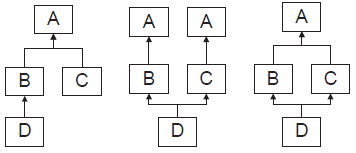
\includegraphics[width=0.47\textwidth]{Hierarchies.png}
  \caption{Single inheritance, repeated multiple inheritance and virtual multiple inheritance}
  \label{fig:hierarchy}
\end{figure}

\noindent
Note that the above picture portrais subobject relatedion, not the inheritance.

The notion of subobject has been formalized before~\cite{RF95,WNST06,RDL11}.
We follow here the presentation of Ramamanandro et al~\cite{RDL11}.

A base class subobject of a given complete object is represented by a pair 
$\sigma = \langle h,l\rangle$ with $h \in \{\mathrm{Repeated},\mathrm{Shared}\}$ representing the 
kind of inheritance (single inheritance is $\mathrm{Repeated}$ with one base class) and $l$ 
representing the path in a non-virtual inheritance graph.

A predicate $C\leftY\sigma\rightY A$ they introduce means that $\sigma$ 
designates a subobject of static type $A$ within the most derived object of 
type $C$.

A class that declares or inherits a virtual function is called a 
\emph{polymorphic class}~\cite[\textsection 10.3]{C++0x}. The C++ ABI in turn defines 
\emph{dynamic class} to be a class requiring a virtual table pointer (because it 
or its bases have one or more virtual member functions or virtual base classes). 
A polymorphic class is thus a dynamic class by definition.

A \emph{virtual table pointer} (vtbl-pointer) is a member of object's layout 
pointing to a virtual table. A \emph{virtual table} is a table of information used 
to dispatch virtual functions, access virtual base class subobjects, and to 
access information for \emph{RunTime Type Identification} (RTTI). Because of repeated
inheritance, an object of given type may have several vtbl-pointers in it. Each 
such pointer corresponds to one of the polymorphic base classes. Given an object 
$a$ of static type $A$ that has $k$ vtbl-pointers in it, we will use the same 
notation we use for regular fields to refer them: $a.\textit{vtbl}_i$.

A \emph{primary base class} for a dynamic class is the unique base class (if any) 
with which it shares the virtual table pointer at offset 0. The data layout 
procedure for non-POD types described in \textsection2.4 of the C++ ABI~\cite{C++ABI} 
requires dynamic classes either to allocate vtable pointer at offset 0 or share 
the virtual table pointer from its primary base class, which is by definition at 
offset 0. For our purpose this means that we can rely on a virtual table pointer 
always being present at offset 0 for all dynamic classes, and thus for all polymorphic 
classes.

\begin{lemma}
In an object layout that adheres to the C++ ABI, a polymorphic class always has a 
virtual table pointer at offset 0.
\label{lem:vtbl}
\end{lemma}

\noindent
Knowing how to extract a vtbl-pointer as well as that all the objects of the 
same most derived type share the same vtbl-pointers, the idea is to use their 
values to uniquely identify the type and subobject within it. Unfortunately 
nothing in the C++ ABI states these pointers should be unique. A popular 
optimization technique lets the compiler share the virtual table of a derived 
class with its primary base class as long as the derived class that does not 
override any virtual methods. Use of such optimization will violate the 
uniqueness of vtbl-pointers; however, we show below that in the presense of 
RTTI, a C++ ABI-compliant implementation is guaranteed to have different values 
of vtbl-pointers in different subobjects.

%C++ standard requires an argument of \code{dynamic_cast} to be a pointer to or 
%an lvalue of a polymorphic type when performing \emph{downcast} -- a cast from 
%base to derived~\cite[\textsection 5.2.7-6]{C++0x}. We can thus always safely 
%extract virtual table pointer from offset 0 of any valid argument to 
%\code{dynamic_cast}.

%Similarly, each class that has virtual member functions or virtual bases has an 
%associated set of virtual tables. There may be multiple virtual tables for a 
%particular class, if it is used as a base class for other classes. However, the 
%virtual table pointers within all the objects (instances) of a particular 
%most-derived class point to the same set of virtual tables.

The exact content of the virtual table is not important for our discussion, but 
we would like to point out a few fields in it. The following definitions are 
copied verbatim from the C++ ABI~\cite[\textsection 2.5.2]{C++ABI}:

\begin{itemize}
\setlength{\itemsep}{0pt}
\setlength{\parskip}{0pt}
\item The \emph{typeinfo pointer} points to the typeinfo object used for RTTI. 
      It is always present.  
\item The \emph{offset to top} holds the displacement to the top of the object 
      from the location within the object of the virtual table pointer that 
      addresses this virtual table, as a \code{ptrdiff_t}. It is always present.
\item \emph{Virtual Base (vbase) offsets} are used to access the virtual bases 
      of an object. Such an entry is added to the derived class object address 
      (i.e. the address of its virtual table pointer) to get the address of a 
      virtual base class subobject. Such an entry is required for each virtual 
      base class.
\end{itemize}

\noindent
Given a virtual table pointer \code{vtbl}, we will refer to these fields as 
\code{rtti(vtbl)}, \code{off2top(vtbl)} and \code{vbase(vtbl)} respectively. 
We will also assume presence of a function $\mathit{offset}(\sigma)$ that defines the 
offset of the base class identified by the end of the path $\sigma$ within a 
class identified by its first element.

\begin{theorem}
In an object layout that adheres to the C++ ABI with present runtime type 
information, the equality of virtual table pointers of two objects of the same 
static type implies that they both belong to subobjects with the same 
inheritance path in the same most-derived type.
\begin{eqnarray*}
    \forall a_1, a_2 : A\ |\ a_1\in C_1\leftY\sigma_1\rightY A \wedge a_2\in C_2\leftY\sigma_2\rightY A \\
    a_1.\textit{vtbl}_i = a_2.\textit{vtbl}_i \Rightarrow C_1 = C_2 \wedge \sigma_1 = \sigma_2
\end{eqnarray*}
\label{thm:vtbl}
\end{theorem}
\begin{proof}
Let us assume first $a_1.\textit{vtbl}_i = a_2.\textit{vtbl}_i$ but $C_1 \neq C_2$. In this case we 
have \code{rtti}$(a_1.\textit{vtbl}_i) = $\code{rtti}$(a_2.\textit{vtbl}_i)$. By definition 
\code{rtti}$(a_1.\textit{vtbl}_i) = C_1$ while \code{rtti}$(a_2.\textit{vtbl}_i) = C_2$, which 
contradicts that $C_1 \neq C_2$. Thus $C_1 = C_2 = C$.

Let us assume now that $a_1.\textit{vtbl}_i = a_2.\textit{vtbl}_i$ but $\sigma_1 \neq \sigma_2$. 
Let $\sigma_i=\langle h_i,l_i\rangle,i=1,2$ 

If $h_1 \neq h_2$ then one of them refers to a virtual base while the other to a 
repeated one. Assuming $h_1$ refers to a virtual path, \code{vbase}$(a_1.\textit{vtbl}_i)$ 
has to be defined inside the vtable according to the ABI, while 
\code{vbase}$(a_2.\textit{vtbl}_i)$ -- should not. This would contradict again that both 
$vtbl_i$ refer to the same virtual table.

We thus have $h_1 = h_2 = h$. If $h = \mathrm{Shared}$ then there is only one path to 
such $A$ in $C$, which would contradict $\sigma_1 \neq \sigma_2$. 
If $h = \mathrm{Repeated}$ then we must have that $l_1 \neq l_2$. In this case let $k$ be 
the first position in which they differ: 
$l_1^j=l_2^j \forall j<k \wedge l_1^k\neq l_2^k$. Since our class $A$ is a base 
class for classes $l_1^k$ and $l_2^k$, both of which are in turn base classes of 
$C$, the object identity requirement of C++ requires that the relevant subobjects 
of type $A$ have different offsets within class $C$: 
$\mathit{offset}(\sigma_1)\neq \mathit{offset}(\sigma_2)$ However 
$\mathit{offset}(\sigma_1)=$\code{off2top}$(a_1.\textit{vtbl}_i)=$\code{off2top}$(a_2.\textit{vtbl}_i)=\mathit{offset}(\sigma_2)$ 
since $a_1.\textit{vtbl}_i = a_2.\textit{vtbl}_i$, which contradicts that the offsets are different.
\end{proof}

\noindent
Conjecture in the other direction is not true in general as there may be 
duplicate virtual tables for the same type present at run-time. This happens in 
many C++ implementations in the presence of DLLs as the same class compiled into 
executable and into a DLL it loads may have identical virtual tables inside the 
executable's and DLL's binaries.

Note also that we require both static types to be the same. Dropping this 
requirement and saying that equality of vtbl-pointers also implies equality of 
the static types is not true in general because a derived class will share the 
vtbl-pointer with its primary base class (see Lemma~\ref{lem:vtbl}). The theorem 
can be reformulated, however, stating that one static type will necessarily have 
to be a subtype of the other. The current formulation is sufficient for our 
purposes, while reformulation would have required more elaborate discussion of 
the algebra of subobjects~\cite{RDL11}, which we touch only briefly.

\begin{corollary}
Results of \code{dynamic_cast} can be reapplied to a different instance from 
within the same subobject. 

$\forall A,B \forall a_1, a_2 : A\ |\ a_1.\textit{vtbl}_i = a_2.\textit{vtbl}_i \Rightarrow$ \\
\code{dynamic_cast<B>}$(a_1).\textit{vtbl}_j = $\code{dynamic_cast<B>}$(a_2).\textit{vtbl}_j \vee$ \\
\code{dynamic_cast<B>}$(a_1)$ throws $\wedge$ \code{dynamic_cast<B>}$(a_2)$ throws.
\label{crl:vtbl}
\end{corollary}

\noindent
During construction and deconstruction of 
an object, the value of a given vtbl-pointer may change. In particular, 
that value will reflect the dynamic type of the object to be the type of the 
fully constructed part only. However, this does not affect our reasoning, as during 
such transition we also treat the object to have the type of its fully 
constructed base only. Such interpretation is in line with the C++ semantics for 
virtual function calls and the use of RTTI during construction and destruction of an 
object. Once the complete object is fully constructed, the value of the 
vtbl-pointer will remain the same for the lifetime of the object.

\subsection{Memoization Device}
\label{sec:memdev}

Let us look at a slightly more general problem than type switching. Consider a 
generalization of the switch statement that takes predicates on a subject as its 
clauses and executes the first statement $s_i$ whose predicate is enabled: 

\begin{lstlisting}
switch (x)
{
    case P1(x): s1;
    ...
    case Pn(x): sn;
}
\end{lstlisting}

\noindent
Assuming that predicates depend only on $x$ and nothing else as well as that 
they do not involve any side effects, we can be sure that the next time we come 
to such a switch with the same value, the same predicate will be enabled 
first. Thus, we would like to avoid evaluating predicates and jump straight to 
the statement it guards. In a way we would like the switch to  memoize which 
case is enabled for a given value of $x$.

The idea is to generate a simple cascading-if statement interleaved with jump 
targets and instructions that associate the original value with enabled target. 
The code before the statement looks up whether the association for a given value 
has already been established, and, if so, jumps directly to the target; otherwise 
the sequential execution of the cascading-if is started. To ensure 
that the actual code associated with the predicates remains unaware of this 
optimization, the code preceeding it after the target must re-establish any 
invariant guaranteed by sequential execution (\textsection\ref{sec:vtblmem}).

The above code can easily be produced in a compiler setting, but producing it in 
a library setting is a challenge. Inspired by Duff's Device~\cite{Duff}, 
we devised a construct that we call \emph{Memoization Device} that does just 
that in standard C++:

\begin{lstlisting}
typedef decltype(x) T;
static std::unordered_map<T,int> jump_target_map;

switch (int& target = jump_target_map[x])
{
default: // entered when we have not seen x yet
    if (P1(x)) { target = 1;   case 1: s1; } else 
    if (P2(x)) { target = 2;   case 2: s2; } else
 ...
    if (Pn(x)) { target = @$n$@; case @$n$@: sn; } else
                target = @$n+1$@;
case @$n+1$@: // none of the predicates is true on x
}
\end{lstlisting}

\noindent
The static \code{jump_target_map} hash table will be allocated upon first entry 
to the function. The map is initially empty and according to its logic, 
request for a key $x$ not yet in the map will result in allocation of a 
new entry with its associated data default initialized (to 0 for int). Since 
there is no case label 0 in the switch, the default case will be taken, which, in 
turn, will initiate sequential execution of the interleaved cascading-if 
statement. Assignments to \code{target} effectively establish association 
between value $x$ and corresponding predicate, since \code{target} is just a 
reference to \code{jump_target_map[x]}. The last assignment records absence of 
enabled predicates for the value.

The sequential execution of the cascading-if statement will keep checking 
predicates $P_j(x)$ until the first predicate $P_i(x)$ that returns true. By 
assigning $i$ to \code{target} we will effectively associate $i$ with $x$ since 
\code{target} is just a reference to \code{jump_target_map[x]}. This association 
will make sure that the next time we are called with the value $x$ we will jump 
directly to the label $i$. When none of the predicates returns true, we will 
record it by associating $x$ with $N+1$, so that the next time we can jump 
directly to the end of the switch on $x$. 

The above construct effectively gives the entire statement first-fit semantics. 
In order to evaluate all the statements whose predicates are true, and thus 
give the construct all-fit semantics, we might want to be able to preserve the 
fall-through behavior of the switch. In this case we can still skip the initial 
predicates returning false and start from the first successful one. This can be 
easily achieved by removing all else statements and making if-statements 
independent as well as wrapping all assignments to \code{target} with a condition, 
to make sure only the first successful predicate executes it:

\begin{lstlisting}
    if (Pi(x)) { if (target == 0) target = @$i$@; case @$i$@: si; }
\end{lstlisting}

\noindent
Note that the protocol that has to be maintained by this structure does not 
depend on the actual values of case labels. We only require them to be 
different and include a predefined default value. The default clause can be 
replaced with a case clause for the predefined value, however keeping the default  
clause results in a faster code. A more important performance consideration is to 
keep the values close to each other. Not following this rule might result in a 
compiler choosing a decision tree over a jump table implementation of the 
switch, which in our experience significantly degrades the performance.

The first-fit semantics is not an inherent property of the memoization device however. 
Assuming that the conditions are either mutually exclusive or imply one another, we 
can build a decision-tree-based memoization device that will effectively have 
\emph{most-specific} semantics -- an analog of best-fit semantics in predicate 
dispatching~\cite{ErnstKC98}.

Imagine that the predicates with the numbers $2i$ and $2i+1$ are mutually exclusive and 
each imply the value of the predicate with number $i$ i.e. $\forall x \in \mathsf{Domain}(P)$
\begin{eqnarray*}
P_{2i+1}(x)\rightarrow P_i(x) \wedge P_{2i}(x)\rightarrow P_i(x) \wedge \neg(P_{2i+1}(x) \wedge P_{2i}(x))
\end{eqnarray*}
\noindent
The following decision-tree based memoization device will execute the statement 
$s_i$ associated with the \emph{most-specific} predicate $P_i$ (i.e. the 
predicate that implies all other predicates true on $x$) that evaluates to true or will 
skip the entire statement if none of the predicates is true on $x$.

\begin{lstlisting}
switch (int& target = jump_target_map[x])
{
default:
    if (P1(x)) {
        if (P2(x)) {
            if (P4(x)) { target = 4; case 4: s4; } else
            if (P5(x)) { target = 5; case 5: s5; } 
            target = 2; case 2: s2;
        } else
        if (P3(x)) {
            if (P6(x)) { target = 6; case 6: s6; } else
            if (P7(x)) { target = 7; case 7: s7; } 
            target = 3; case 3: s3;
        }
        target = 1; case 1: s1;
    } else {
        target = 0; case 0:   ;
    }
}
\end{lstlisting}

\noindent
An example of predicates that satisfy this condition are class membership tests
where the truth of a predicate that tests membership in a derived class implies 
the truth of a predicate that tests membership in its base class. Our library 
solution prefers the simpler cascading-if approach only because the necessary 
structure of the code can be laid out directly with macros. A compiler solution 
will use the decision-tree approach whenever possible to lower the cost of the 
first match from linear in case's number to logarithmic as seen in Figure\ref{fig:DCastVis1}.

When the predicates do not satisfy the implication or mutual exclusion properties 
mentioned above, a compiler of a language based on predicate dispatching would 
typically issue an ambiguity error. Some languages might choose to resolve it 
according to lexical or some other ordering. In any case, the presence of 
ambiguities or their resolution has nothing to do with memoization device 
itself. The latter only helps optimize the execution once a particular choice of 
semantics has been made and code implementing it has been laid out.

The main advantage of the memoization device is that it can be built around 
almost any code, providing that we can re-establish the invariants, guaranteed 
by sequential execution. Its main disadvantage is the size of the hash table 
that grows proportionally to the number of different values seen. Fortunately, 
the values can often be grouped into equivalence classes, such that values in 
the same class do not change the predicate. The map can then associate the 
equivalence class of a value with a target instead of associating the value with 
it. The next subsection does exactly that for polymorphic objects.

\subsection{Vtable Pointer Memoization}
\label{sec:vtblmem}

The memoization device can almost immediately be used for multi-way type testing by 
using \code{dynamic_cast<Di>} as a predicate $P_i$. This cannot be considered a 
type switching solution, however, as one would expect to also have a reference 
to the uncovered type. Using a \code{static_cast<Di>} upon successful type test 
would have been a solution if we did not have multiple inheritance. It certainly 
can be used as such in languages with only single inheritance. For the fully 
functional C++ solution, we combine the memoization device with the properties 
of virtual table pointers into a \emph{Vtable Pointer Memoization} technique.

We saw that vtbl-pointers uniquely determine the subobject within an object 
(Theorem~\ref{thm:vtbl}), while the result of a \code{dynamic_cast} can be reapplied 
from the same subobject (Corollary~\ref{crl:vtbl}). The idea is thus to group 
all the objects according to the value of their vtbl-pointer and associate both 
target and the required offset with it through memoization device:

\begin{lstlisting}
typedef std::pair<ptrdiff_t,size_t> type_switch_info;
static std::unordered_map<intptr_t, type_switch_info> jump_target_map;
intptr_t          vtbl = *reinterpret_cast<const intptr_t*>(p);
type_switch_info& info = jump_target_map[vtbl];
const void*       tptr; 
switch (info.second) ...
\end{lstlisting}

\noindent
We use the virtual table pointer extracted from a polymorphic object pointed to 
by \code{p} as a key for association. The value stored along the key in 
association now keeps both: the target for the switch as well as a memoized 
offset for dynamic cast. 

The code for the $i^{th}$ case now evaluates the required offset on the first 
entry and associates it along the target with the vtbl-pointer of the subject.
The call to \code{adjust_ptr<Di>} re-establishes the invariant that 
\code{matched} is a properly-casted reference to type \code{Di} of the subject 
\code{p}.
%The condition of the inner if-statement is only needed to implement the 
%sequential all-fit semantics and can be removed when fall-through behavior is 
%not required.

\begin{lstlisting}
    if (tptr = dynamic_cast<const Di*>(p)) {
        if (info.second == 0) { // supports fall-through
            info.first  = intptr_t(tptr)-intptr_t(p); // offset
            info.second = @$i$@; // jump target
        }
case @$i$@: // @$i$@ is a constant here - clause's position in switch
        auto matched = adjust_ptr<Di>(p,info.first); 
        si;
    }
\end{lstlisting}

\noindent
The main condition remains the same. We keep checking for the first initialization 
because we allow fall-through semantics here, letting the user break from the 
switch when needed. Upon first entry we compute the offset that the dynamic cast 
performed and save it together with target associated to the virtual table 
pointer. On the next iteration we will jump directly to the case label and 
restore the invariant of \code{matched} being a properly-casted reference to the 
derived object.

The use of dynamic cast makes a huge difference in comparison to the use of 
static cast we dismissed above. First of all the C++ type system is much more 
restrictive about the static cast and many cases where it is not allowed can 
still be handled by dynamic cast. Examples of these include downcasting from an 
ambiguous base class or cross-casting between unrelated base classes.

An important benefit we get from this optimization is that we do not store the 
actual values (pointers to objects) in the hash table anymore, but group them 
into equivalence classes based on their virtual table pointers. The number of 
such pointers in a program is always bound by $O(|A|)$, where $A$ represents the 
static type of an object, while $|A|$ represents the number of classes directly 
or indirectly derived from $A$. The linear coefficient hidden in big-o notation 
reflects possibly multiple vtbl-pointers in derived classes due to the use of 
multiple inheritance.

\begin{figure}[htbp]
  \centering
    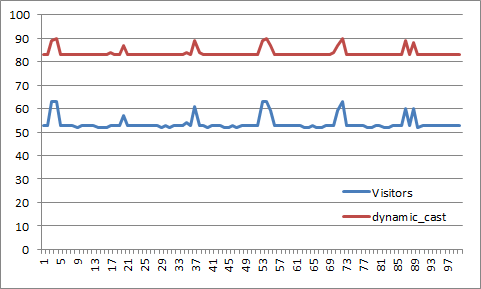
\includegraphics[width=0.47\textwidth]{DCast-vs-Visitors3.png}
  \caption{Time to uncover i\textsuperscript{th} case. X-axis - case i; Y-axis - cycles per iteration}
  \label{fig:DCastVis3}
\end{figure}

The most important benefit of this optimization, however, is the constant time 
on average used to dispatch each of the case clauses, regardless of their 
position in the type switch. The net effect of this optimization can be seen in Figure~\ref{fig:DCastVis3}. 
We can see that the time does not increase with the position of the case we are 
handling. The spikes represent activities on computer during measurement and are 
present in both measurements. 
The constant time on average comes from the average complexity 
of accessing an element in an \code{unordered_map}, while its worst complexity can 
be proportional to the size of the map. We show in the next section, however, 
that most of the time we will be bypassing traditional access to elements of the 
map, because, as-is, the type switch is still about 50\% slower than the visitor 
design pattern.

Note that we can apply the reasoning of \textsection\ref{sec:memdev} and change 
the first-fit semantics of the resulting match statement into a best-fit 
semantics simply by changing the underlying cascading-if structure with decision 
tree. A compiler implementation of a type switch based on Vtable Pointer 
Memoization will certainly take advantage of this optimization to cut down the 
cost of the first run on a given vtbl-pointer, when the actual memoization happens.

\subsubsection{Structure of Virtual Table Pointers}
\label{sec:sovtp}

Virtual table pointers are not entirely random addresses in memory and have 
certain structure when we look at groups of those that are associated with 
classes related by inheritance. Let us first look at some vtbl pointers that 
were present in some of our tests. The 32-bit pointers are shown in binary form 
(lower bits on the right) and are sorted in ascending order:

\begin{verbatim}
00000001001111100000011001001000
00000001001111100000011001011100
00000001001111100000011001110000
 ...
00000001001111100000011111011000
00000001001111100000011111101100
\end{verbatim}

Virtual table pointers are not constant values and are not even guaranteed to be 
the same between different runs of the same application. Techniques like 
\emph{address space layout randomization} or simple \emph{rebasing} of the entire 
module are likely to change these values. The relative distance between them is 
likely to remain the same though as long as they come from the same module.

Comparing all the vtbl pointers that are coming through a given match statement 
we can trace ar run time the set of bits in which they do and do not differ. 
For the above example it may look as \texttt{00000001001111100000X11XXXXXXX00} 
where positions marked with X represent bits that are different in some vtbl 
pointers.

When a DLL is loaded it may have its own copy of vtables for classes also used 
in other modules as well as vtables for classes it introduces. Comparing 
similarly all vtbl pointers coming only from this DLL we can get a different 
pattern \\ \texttt{01110011100000010111XXXXXXXXX000} and when compared over all 
the loaded modules the pattern will likely becomes something like 
\texttt{0XXX00X1X0XXXXXX0XXXXXXXXXXXXX00}.

The common bits on the right come from the virtual table size and alignment 
requirements, and, depending on compiler, configuration, and class hierarchy could 
easily vary from 2 to 6 bits. Because the vtbl-pointer under the C++ ABI points into 
an array of function pointers, the alignment requirement of 4 bytes for those 
pointers on a 32-bit architecture is what makes at least the last 2 bits to be 0. 
For our purpose the exact number of bits on the right is not important as we 
evaluate this number at run time based on vtbl-pointers seen so far. Here we only 
would like to point out that there would be some number of common bits on the 
right.

Another observation we made during our experiments with the vtbl-pointers of various 
existing applications was that the values of the pointers where changing more 
frequently in the lower bits than in the higher ones. We believe that this was 
happening because programmers tend to group multiple derived classes in the same 
translation unit so the compiler was emitting virtual tables for them close to 
each other as well. 

Note that derived classes that do not introduce their own virtual functions 
(even if they override some existing ones) are likely to have virtual tables of 
the same size as their base class. Even when they do add new virtual functions, 
the size of their virtual tables can only increase relative to their base 
classes. This is why the difference between many consecutive vtbl-pointers that 
came through a given match statement was usually constant or very slightly 
different.

The changes in higher bits were typically due to separate compilation and 
especially due to dynamically loaded modules. When a DLL is loaded, it may have 
its own copies of vtables for classes that are also used in other modules, in addition to 
vtables for classes it introduces. Comparing all vtbl-pointers coming only from 
that DLL we can get a different pattern \texttt{01110011100000010111XXXXXXXXX000} 
and when compared over all the loaded modules the pattern will likely become 
something like \texttt{0XXX00X1X0XXXXXX0XXXXXXXXXXXXX00}. Overall they were not 
changing the general tendency we saw: smaller bits were changing more frequently 
than larger ones, with the exception of the lowest common bits, of course.

These observations made virtual table pointers of classes related by inheritance 
ideally suitable for indexing -- the values obtained by throwing away the common 
bits on the right were compactly distributed in small disjoint ranges. We use 
those values to address a cache built on top of the hash table in order to 
eliminate a hash table lookup in most of the cases.  The important 
guarantee about the validity of the cached hash table references comes from the 
C++0x standard, which states that ``insert and emplace members shall not affect 
the validity of references to container elements''~\cite[\textsection 
23.2.5(13)]{C++0x}. 

Depending on the number of actual collisions that happen in the cache, our 
vtable pointer memoization technique can come close to, and even outperform, the 
visitor design pattern. The numbers are, of course, averaged over many runs as 
the first run on every vtbl-pointer will take an amount of time as shown in 
Figure\ref{fig:DCastVis1}. We did however test our technique on real code and 
can confirm that it does perform well in the real-world use cases.

The information about jump targets and necessary offsets is just an example of 
information we might want to be able to associate with, and access via, virtual 
table pointers. Our implementation of \code{memoized_cast} from 
\textsection\ref{sec:memcast} effectively reuses this general data structure with 
a different type of element values. We thus created a generic reusable class 
\code{vtblmap<T>} that maps vtbl-pointers to elements of type T. We will refer 
to the combined cache and hash-table data structure, extended with the logic for 
minimizing conflicts presented below, as a \emph{vtblmap} data structure.

\subsubsection{Minimization of Conflicts}
\label{sec:moc}

The small number of cycles that the visitor design pattern needs to uncover a 
type does not let us put too sophisticated cache indexing mechanisms into the 
critical path of execution. This is why we limit our indexing function to shifts 
and masking operations as well as choose the size of the cache to be a power of 2.

Throughout this section by \emph{collision} we will call a run-time condition in 
which the cache entry of an incoming vtbl pointer is occupied by another vtbl-pointer.
Collision requires vtblmap to fetch the data associated with the new 
vtbl-pointer from a slower hash-table and, under certain conditions, reconfigure 
cache for better performance. By \emph{conflict} we will call a different 
run-time condition under which given cache configuration maps two or more vtbl 
pointers to the same cache location. Presence of conflict does not necessarily 
imply presence of collisions, but collisions can only happen when there is a 
conflict. In the rest of this section we devise a mechanism that tries to 
minimize the amount of conflicts in a hope that it will also decrease the amount 
of actual collisions.

Given $n$ vtbl-pointers we can always find a cache size that will render no 
conflicts between them. The necessary size of such a cache, however, can be too 
big to justify the use of memory. This is why, in our current implementation, we 
always consider only 2 different cache sizes: $2^k$ and $2^{k+1}$ where 
$2^{k-1} < n \leq 2^k$. This guarantees that the cache size is never more than 4 
times bigger than the minimum required cache size.

During our experiments, we noticed that often the change in the smallest 
different bit happens only in a few vtbl-pointers, which was effectively 
cutting the available cache space in half. To overcome this problem, we let the 
number of bits by which we shift the vtbl-pointer vary further and compute it in 
a way that minimizes the number of conflicts.

To avoid doing any computations in the critical path, \code{vtblmap} only 
recomputes the optimal shift and the size of the cache when an actual collision 
happens. In order to avoid constant recomputations when conflicts are unavoidable, 
we add an additional restriction of only reconfiguring the optimal parameters if 
the number of vtbl-pointers in the \code{vtblmap} has increased since the last 
recomputation. Since the number of vtbl-pointers is of the order $O(|A|)$, where 
$A$ is the static type of all vtbl-pointers coming through a \code{vtblmap}, the 
restriction assures that reconfigurations will not happen infinitely often.

To minimize the number of recomputations even further, our library communicates 
to the \code{vtblmap}, through its constructor, the number of case clauses in 
the underlying match statement. We use this number as an estimate of the expected 
size of the \code{vtblmap} and pre-allocate the cache according to this estimated 
number. The cache is still allowed to grow based on the actual number of 
vtbl-pointers that comes through a \code{vtblmap}, but it never shrinks from the
initial value. This improvement significantly minimizes the number of collisions 
at early stages, as well as the number of possibilities we have to consider 
during reconfiguration.

The above logic of \code{vtblmap} always chooses the configuration that renders 
no conflicts, when such a configuration is possible during recomputation of 
optimal parameters. When this is not possible, it is natural to prefer collisions 
to happen on less-frequent vtbl-pointers.

We studied the frequency of vtbl-pointers that come through various match statements
of a C++ pretty-printer that we implemented on top of the Pivot 
framework~\cite{Pivot09} using our pattern-matching library. We ran the 
pretty-printer on a set of C++ standard library headers and then ranked all the  
classes from the most-frequent to the least-frequent ones, on average. The 
resulting probability distribution is shown with a thicker line in 
Figure\ref{fig:PowerLaw}.

\begin{figure}[htbp]
  \centering
    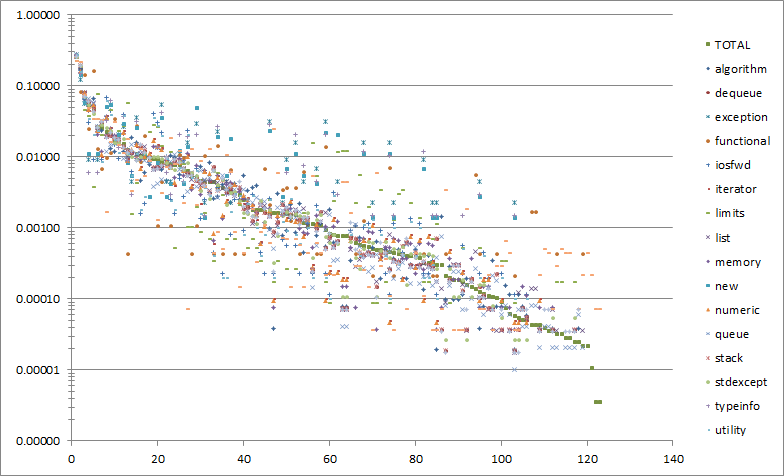
\includegraphics[width=0.47\textwidth]{std-lib-power-law-distributions.png}
  \caption{Probability distribution of various nodes in Pivot framework}
  \label{fig:PowerLaw}
\end{figure}

Note that Y-Axis is using logarithmic scale, suggesting that the resulting 
probability has power-law distribution. This is likely to be a specifics of our 
application, nevertheless, the above picture demonstrates that frequency of certain 
classes can be larger than the overall frequency of all the other classes. In 
our case, the two most frequent classes were representing the use of a variable in 
a program, and their combined frequency was larger than the frequency of all the 
other nodes. Naturally, we would like to avoid conflicts on such classes in the 
cache, when possible.

Let us assume that a given \code{vtblmap} contains a set of vtbl pointers 
$V = \{v_1, ... , v_n\}$ with known probabilities $p_i$ of occuring. For a cache 
of size $2^k$ and a shift by $l$ bits we get a cache-indexing function 
$f_{lk} : V \rightarrow [0..2^k-1]$ defined as $f_{lk}(v_i) = (v_i \gg l) \& (2^k-1)$.
To calculate the probability of conflict for a given $l$ and $k$ parameters, let 
us consider $j^{th}$ cache cell and a subset $V^j_{lk}=\{v \in V | f_{lk}(v)=j\}$. 
When the size of this subset $m=|V^j_{lk}|$ is greater than 1, we have a 
potential conflict as subsequent request for a vtbl pointer $v''$ might be 
different from the vtbl pointer $v'$ currenly stored in the cell $j$. Within the 
cell only the probability of not having a conflict is the probability of both 
values $v''$ and $v'$ be the same:
\begin{eqnarray*}
P(v''=v')=\sum\limits_{v_i \in V^j_{lk}}P(v''=v_i)P(v'=v_i)=\sum\limits_{v_i \in V^j_{lk}}P^2(v_i|V^j_{lk})=\\
=\sum\limits_{v_i \in V^j_{lk}}\frac{P^2(v_i)}{P^2(V^j_{lk})}=
\sum\limits_{v_i \in V^j_{lk}}\frac{p_i^2}{(\sum\limits_{v_{i'} \in V^j_{lk}}p_{i'})^2}=
\frac{\sum\limits_{v_i \in V^j_{lk}}p_i^2}{(\sum\limits_{v_{i} \in V^j_{lk}}p_{i})^2}
\end{eqnarray*}

The probability of having a conflict among the vtbl pointers of a given cell is 
thus one minus the above value:

\begin{eqnarray*}
P(v''\neq v')=1-\frac{\sum\limits_{v_i \in V^j_{lk}}p_i^2}{(\sum\limits_{v_{i} \in V^j_{lk}}p_{i})^2}
\end{eqnarray*}

To obtain probability of conflict given any vtbl pointer and not just the one 
from a given cell we need to sum up the above probabilities of conflict within a 
cell multiplied by the probability of vtbl pointer fall into that cell:

\begin{eqnarray*}
P_{lk}^{conflict}=\sum\limits_{j=0}^{2^k-1}P(V^j_{lk})(1-\frac{\sum\limits_{v_i \in V^j_{lk}}p_i^2}{(\sum\limits_{v_{i} \in V^j_{lk}}p_{i})^2})=\\
=\sum\limits_{j=0}^{2^k-1}(\sum\limits_{v_{i} \in V^j_{lk}}p_{i})(1-\frac{\sum\limits_{v_i \in V^j_{lk}}p_i^2}{(\sum\limits_{v_{i} \in V^j_{lk}}p_{i})^2})
\end{eqnarray*}

Our reconfiguration algorithm then iterates over possible values of $l$ and $k$ 
and chooses those that minimize the overal probability of conflict $P_{lk}^{conflict}$.
The only data still missing are the actual probabilities $p_i$ used by the above 
formula. They can be approximated in many different ways.

Besides probability distribution on all the tests, Figure~\ref{fig:PowerLaw} 
shows probabilities of a given node on each of the tests. The X-Axis in this 
case represents the ordering of all the nodes according to their overall rank 
of all the tests combined. As can be seen from the picture, the shape of each 
specific test's distribution still mimics the overal probability distribution. 
With this in mind we can simply let the user assign probabilities to each of the 
classes in the hierarchy and use these values during reconfiguration. The 
practical problem we came accross with this solution was that we wanted these 
probabilities be inheritable as Pivot separates interface and implementation 
classes and we prefered the user to define them on interfaces rather than on 
implementation classes. The easiest way to do so wast to write a dedicated 
function that would return the probabilities using a match statement. 
Unfortunately such a function will introduce a lot of overhead as it will 
ideally only be used very few times (since we try to minimize the amount of 
reconfiguration) and thus not be using memoized jumps but rather slow 
cascading-if.

A simpler and likely more precise way of estimating $p_i$ would be to count 
frequencies of each vtbl pointers directly inside the \code{vtblmap}. This 
introduces an overhead of an increment into the critical path of execution, but 
according to our tests was only degrading the overal performance by 1-2\%.
Instead, it was compensating with a smaller amount of conflicts and thus a 
potential gain of performance. We leave the choice of whether the library should 
count frequencies of each vtbl pointer to the user of the library as the 
concrete choice may be to advantage on some class hierarchies and to 
disadvantage on others.

Figure~\ref{fig:Collisions} compares the amount of collisions when frequency 
information is and is not used. The data was gathered from 312 tests on multiple 
match statements present in Pivot's C++ pretty printer when it was ran over 
standard library headers. In 122 of these test both schemes had 0 conflicts and 
these tests are thus not shown on the graph. The remaining tests where ranked by 
the amount of conflicts in the scheme that does not utilize frequency information.

\begin{figure}[htbp]
  \centering
    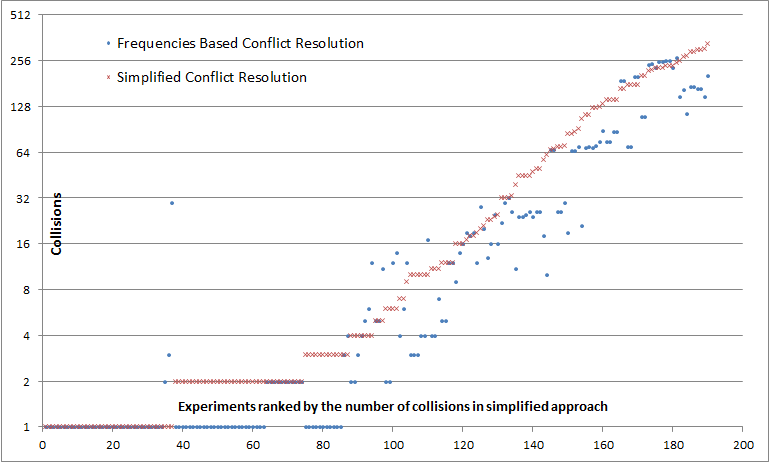
\includegraphics[width=0.47\textwidth]{CollisionsWithAndWithoutFrequencies.png}
  \caption{Decrease in number of collisions when probabilities of nodes are taken into account}
  \label{fig:Collisions}
\end{figure}

As can be seen from the graph, both schemes render quite low amount of 
collisions given that there was about 57000 calls in the rightmost test having 
the largest amount of conflicts. Taking into account that the Y-axis has 
logarithmic scale, the use of frequency information in many cases decreased the 
amount of conflicts by a factor of 2. The handfull of cases where the use of 
frequency increased the number of conflicts can be explained by the fact that 
the optimal values are not recomputed after each conflict, but after several 
conflicts and only if the amount of vtbl pointers in the vtblmap increased. These 
extra conditions sacrify optimality of parameters at any given time for the amount 
of times they are recomputed. By varying the number of conflicts we are willing 
to tolerate before reconfiguration we can decrease the number of conflicts by 
increasing the amount of recomputations and vise versa. From our experience, 
however, we saw that the drop in the number of conflicts was not translating 
into a proportional drop in execution time, while the amount of reconfigurations 
was proportional to the increase in execution time. This is why we choose to 
tolerate a relatively large amount of conflicts before recomputation just to 
keep the amount of recomputations low.

\section{Solution for Tagged Classes}
\label{sec:cotc}

The memoization device outlined in \textsection\ref{sec:memdev} can, in principle, also be 
applied to tagged classes. The dynamic cast will be replaced by a small 
compile-time template meta-program that checks whether the class associated with 
the given tag is derived from the target type of the case clause. If so, a static 
cast can be used to obtain the offset.

Despite its straightforwardness, we felt that it should be possible to do better 
than the general solution, given that each class is already identified with a 
dedicated constant known at compile time.

As we mentioned in \textsection\ref{sec:poets}, the nominal subtyping of C++ 
effectively gives every class multiple types. The idea is thus to associate with 
the type not only its most derived tag, but also the tags of all its base classes.
In a compiler implementation such a list can be stored inside the virtual table 
of a class, while in our library solution it is shared between all the instances 
with the same most derived tag in a less efficient global map, associating the 
tag to its tag list.

The list of tags is topologically sorted according to the subtyping relation 
and terminates with a dedicated value distinct from all the tags. We call such a 
list a \emph{Tag Precedence List} (TPL) as it resembles the \emph{Class 
Precedence List} (CPL) of object-oriented descendants of Lisp (e.g. Dylan, 
Flavors, LOOPS, and CLOS) used there for \emph{linearization} of class 
hierarchies. The classes in CPL are ordered from most specific to least specific 
with siblings listed in the \emph{local precedence order} -- the order of the 
direct base classes used in the class definition. TPL is just an implementation 
detail and the only reason we distinguish TPL from CPL is that in C++ classes 
are often separated into interface and implementation classes and it might so 
happen that the same tag is associated by the user with an interface and several 
implementation classes. 

A type switch below, built on top of a hierarchy of tagged classes, proceeds as 
a regular switch on the subject's tag. If the jump succeeds, we found an exact 
match; otherwise, we get into a default clause that obtains the next tag in the 
tag precedence list and jumps back to the beginning of the switch statement for a 
rematch:

\begin{lstlisting}
    const size_t* taglist = 0;
          size_t  attempt = 0;
          size_t  tag     = object->tag;
ReMatch:
    switch (tag) 
    {
    default:
        if (!taglist) 
            taglist = get_taglist(object->tag);
        tag = taglist[++attempt];
        goto ReMatch;
    case end_of_list: break;
    case bindings<D1>::kind_value: s1; break;
    ...
    case bindings<Dn>::kind_value: sn; break;
    }
\end{lstlisting}

\noindent
The above structure, which we call \emph{TPL Dispatcher}, lets us dispatch to case clauses of the most derived class 
with an overhead of initializing two local variables, compared to a switch on a 
sealed hierarchy. Dispatching to a case clause of a base class will take time 
roughly proportional to the distance between the matched base class and the most 
derived class in the inheritance graph. When none of the base class tags was 
matched, we will necessarily reach the end\_of\_list marker in the tag precedence 
list and thus exit the loop.

Our library automatically builds the function \code{get_taglist} based on the 
\code{BC} or \code{BCS} specifiers that the user specifies in bindings 
(\textsection\ref{sec:bnd}).

To make the behavior clos

\begin{lstlisting}
    if (is_derived_from<Di>(object))
    {
case bindings<Di>::kind_value:
        auto matched = static_cast<Di>(object); 
        si;
    }
\end{lstlisting}


\section{(Ab)using Exceptions for Type Switching}
\label{sec:xpm}

Several authors had noted the relationship between exception handling and type 
switching before~\cite{Glew99,ML2000}. Not surprisingly, the exception handling 
mechanism of C++ can be abused to implement the first-fit semantics of a type 
switch statement. The idea is to harness the fact that catch-handlers in C++ 
essentially use first-fit semantics to decide which one is going to handle a 
given exception. The only problem is to raise an exception with a static type 
equal to the dynamic type of the subject.

To do this, we employ the \emph{polymorphic exception} idiom~\cite{PolyExcept} that 
introduces a virtual function \code{virtual void raise() const = 0;} into the 
base class, overridden by each derived class in syntactically the same way: 
\code{throw *this;}. The \code{Match}-statement then simply calls \code{raise} on its subject, 
while case clauses are turned into catch-handlers.
The exact name of the function is not important, and is communicated to the 
library as \emph{raise selector} with \code{RS} specifier in the same way 
\emph{kind selector} and \emph{class members} are (\textsection\ref{sec:bnd}). 
The \code{raise} member function can be seen as an analog of the \code{accept} 
member function in the visitor design pattern, whose main purpose is to discover 
subject's most specific type. The analog of a call to \code{visit} to communicate 
that type is replaced, in this scheme, with exception unwinding mechanism.

Just because we can, it does not mean we should abuse the exception handling 
mechanism to give us the desired control flow. In the table-driven approach 
commonly used in high-performance implementations of exception handling, the 
speed of handling an exception is sacrificed to provide a zero execution-time 
overhead for when exceptions are not thrown~\cite{Schilling98}. Using exception 
handling to implement type switching will reverse the common and exceptional 
cases, significantly degrading performance. As can be seen in 
Figure\ref{fig:DCastVis1}, matching the type of the first case clause with 
polymorphic exception approach takes more than 7000 cycles and then grows 
linearly (with the position of case clause in the match statement), making it the 
slowest approach. The numbers illustrate why exception handling should only be 
used to deal with exceptional and not common cases.

Despite its total inpracticality, the approach fits well into our unified syntax 
(\textsection\ref{sec:unisyn}) and gave us a very practical idea of harnessing a
C++ compiler to do \emph{redundancy checking} at compile time.

\subsection{Redundancy Checking}
\label{sec:redun}

As discussed in \textsection\ref{sec:bg}, redundancy checking is only applicable 
to first-fit semantics of the match statement, and warns the user of any 
case clause that will never be entered because of a preceding one being more 
general.

We provide a library-configuration flag, which, when defined, effectively turns 
the entire match statement into a try-catch block with handlers accepting the 
target types of the case clauses. This forces the compiler to give warning when 
a more general catch handler preceds a more specific one effectively performing 
redundancy checking for us, e.g.:

\begin{lstlisting}
filename.cpp(55): warning C4286: 'ipr::Decl*' : is caught by 
                  base class ('ipr::Stmt*') on line 42
\end{lstlisting}

\noindent
Note that the message contains both the line number of the redundant case clause (55) 
and the line number of the case clause that makes it redundant (42).

Unfortunately, the flag cannot be always enabled, as the case labels of the underlying 
switch statement have to be eliminated in order to render a syntactically 
correct program. Nevertheless, we found the redundancy checking facility of the 
library extremely useful when rewriting visitor-based code: even though the 
order of overrides in a visitor's implementation does not matter, for some reason 
more general ones were inclined to happen before specific ones in the code we 
looked at. Perhaps programmers are inclined to follow the class declaration order when 
defining and implementing visitors.

A related \emph{completeness checking} -- test of whether a given match 
statement covers all possible cases -- needs to be reconsidered for extensible 
data types like classes, since one can always add a new variant to it. 
Completeness checking in this case may simply become equivalent to ensuring that 
there is either a default clause in the type switch or a clause with the static type 
of a subject as a target type. In fact, our library has an analog of a default 
clause called \code{Otherwise}-clause, which is implemented under the hood 
exactly as a regular case clause with the subject's static type as a target type.

\section{Unified Syntax}
\label{sec:unisyn}

The discussion in this subsection will be irrelevant for a compiler 
implementation, nevertheless we include it because some of the challenges we 
came accross as well as techniques we used to overcome them might show up in 
other active libraries. The problem is that working in a library setting, the 
toolbox of properties we can automatically infer about user's class hierarchy, 
match statement, clauses in it, etc. is much more limited than the set of 
properties a compiler can infer. On one side such additional information may let 
us generate a better code, but on the other side we understand that it is 
important not to overburden the user's syntax with every bit of information she 
can possibly provide us with to generate a better code. Some examples of 
information we can use to generate a better code even in the library setting 
include:

\begin{itemize}
\setlength{\itemsep}{0pt}
\setlength{\parskip}{0pt}
\item Encoding we are dealing with (\textsection\ref{sec:adt})
\item Shape of the class hierarchy: flat/deep, single/multiple inheritance etc.
\item The amount of clauses in the match statement
\item Presense of Otherwise clause in the match statement
\item Presence of extensions in dynamically linked libraries
\end{itemize}

We try to infer the information when we can, but otherwise resort to a usually 
slower default that will work in all or most of the cases. The major source of 
inefficiency comes from the fact that macro resolution happens before any 
meta-programming techniques can be employed and thus the macros have to generate 
a syntactic structure that can essentially handle all the cases as opposed to 
the exact case. Each of the macros involved in rendering the syntactic structure 
of a match statement (e.g. \code{Match}, \code{Case}, \code{Otherwise}) have a 
version identified with a suffix that is specific to a combination of encoding 
and shape of the class hierarchy. By default the macros are resolved to a 
unified version that infers encoding with a template meta-program, but this 
resolution can be overriden with a configuration flag for a more specific 
version when all the match statements in user's program satisfy the requirements 
of that version. The user can also pin-point specific match statement with the 
most applicable version, but we discourage such use as performance differences 
are not big enough to justify the exposure of details.

To better understand what is going on, consider the following examples. Case 
labels for polymorphic base class encoding can be arbitrary, but preferably 
sequential numbers, while the case labels for tagged class and discriminated 
union encodings are the actual kind values associated with concrete variants.
Discriminated union and tagged class encodings can use both types (views in case
of unions) and kind values to identify the target variant, while polymorphic 
base class encoding can only use types for that. The latter encoding requires 
allocation of a static vtblmap in each match statement, not needed by any other 
encoding, while tagged class encoding on non-flat hierarchy requires the use of 
default label of the generated switch statement as well as a dedicated case 
label distinct from all kind values (\textsection\ref{sec:cotc}). 
When merging these and other requirements into a syntactic structure of a 
unified version capable of handling any encoding we essentially always have to 
reserve the use of default label (and thus not use it to generate 
\code{Otherwise}-clause), allocate an extra dedicated case label, introduce  
a loop over base classes used by tagged class encoding etc. This is a clear 
overhead for handling of a discriminated union encoding whose syntactic 
structure only involves a simple switch over kind values and default label to 
implement \code{Otherwise}. To minimize the effects of this overhead we rely on 
compiler's optimizer to inline calls specific to each encoding and either remove 
branching on conditions that will always be true after inlining or elminate dead 
code on conditions that will always be false after inlining. Luckily for us 
today's compilers do a great job in doing just that, rendering our unified 
version only slightly less efficient than the specialized ones. These 
differences can be best seen in Figure\ref{relperf} under corresponding entries 
of \emph{Unified} and \emph{Specialized} columns.

\section{Memoized Dynamic Cast}
\label{sec:memcast}

We saw in Corollary~\ref{crl:vtbl} that the results of \code{dynamic_cast} can 
be reapplied to a different instance from within the same subobject. This leads 
to simple idea of memoizing the results of \code{dynamic_cast} and then using 
them on subsequent casts. In what follows we will only be dealing with the 
pointer version of the operator since the version on references that has a 
slight semantic difference can be easily implemented in terms of the pointer one.

The \code{dynamic_cast} operator in C++ involves two arguments: a value argument 
representing an object of a known static type as well as a type argument 
denoting the runtime type we are querying. Its behavior is twofold: on one hand 
it should be able to determine when the object's most derived type is not a 
subtype of the queried type (or when the cast is ambiguous), while on the other 
it should be able to produce an offset by which to adjust the value argument when it is.

We mimic the syntax of \code{dynamic_cast} by defining:

\begin{lstlisting}
template <typename T, typename S>
inline T memoized_cast(S* p);
\end{lstlisting}

\noindent
which lets the user replace all the uses of \code{dynamic_cast} in the program 
with \code{memoized_cast} with a simple:

\begin{lstlisting}
#define dynamic_cast memoized_cast
\end{lstlisting}

\noindent
It is important to stress that the offset is not a function of the source and target 
types of the \code{dynamic_cast} operator, which is why we cannot simply memoize the 
outcome inside the individual instantiations of \code{memoized_cast}.
The use of repeated multiple inheritance will result in classes having several 
different offsets associated with the same pair of source and target types 
depending on which subobject the cast is performed from. According to 
corollary~\ref{crl:vtbl}, however, it is a function of target type and the value 
of the vtbl-pointer stored in the object, because the vtbl-pointer uniquely 
determines the subobject within the most derived type. Our memoization of the 
results of \code{dynamic_cast} should thus be specific to a vtbl-pointer and the 
target type. 

The easiest way to achieve this would be to use a dedicated global
\code{vtblmap<std::ptrdiff_t>} (\textsection\ref{sec:sovtp}) per each 
instantiation of the \code{memoized_cast}. This, however, will create an 
unnecessarily large amount of vtblmap structures, many of which will be  
duplicating information and repeating the work already done. This will happen 
because instantiations of \code{memoized_cast} with same target but different 
source types can share their vtblmap structures since vtbl pointers of different 
source types are necessarily different according to Theorem~\ref{thm:vtbl}. 

Even though the above solution can be easily improved to allocates a single 
vtblmap per target type, an average application might have a lot of different 
target types. This is especially true for applications that will use our Match 
statement since we use \code{dynamic_cast} under the hood in each case clause. 
Indeed our C++ pretty printer was creating 160 vtblmaps of relatively small size 
each, which was increasing the executable size quite significantly because of 
numerous instantiations as well as noticably slowed down the compilation time.

To overcome the problem we turn each target type into a runtime instantiation 
index of the type and allocate a single \code{vtblmap<std::vector<std::ptrdiff_t>>} 
that associates vtbl pointers with a vector of offsets indexed by target type. 
The slight performance overhead that is brought by this improvement is specific 
to our library solution and would not be present in a compiler implementaion. 
Instead we get a much smaller memory footrpint, which can be made even smaller 
once we recognize the fact that global type indexing may effectively enumerate 
target classes that will never appear in the same Match statement. This will 
result in entries in the vector of offsets that are never used.

Our actual solution uses separate indexing of target types for each source type 
they are used with, and also allocates a different 
\code{vtblmap<std::vector<std::ptrdiff_t>>} for each source type. This lets us 
minimize unused entries within offset vectors by making sure only the plausible 
target types for a given source type are indexed. This solution should be 
suitable for most applications since we expect to have a fairly small 
number of source types for the \code{dynamic_cast} operator and a much larger number 
of target types. For the unlikely case of a small number of target types and large 
number of source types we allow the user to revert to the default behavior with a 
library configuration switch that allocates a single \code{vtblmap} per target type as 
we have already discussed above.

The use of \code{memoized_cast} to implement the \code{Match}-statement potentially reuses the 
results of \code{dynamic_cast} computations across multiple independent match 
statements. This allows leveraging the cost of the expensive first call with a 
given vtbl-pointer even further across all the match statements inside the 
program. The above define, with which a user can easily turn all dynamic casts 
into memoized casts, can be used to speed-up existing code that uses dynamic 
casting without any refactoring overhead.
